\chapter{إنتروبيا التفاعل وطاقته الحرة}\label{ch:b2:reaction-free-energy}

تحوي كمادة التبريد الرياضية كيسًا من الماء وبضع ملاعق من نترات
الأمونيوم. اضغطها فينفجر الكيس الداخلي ويذوب الملح، وفي ثوانٍ تصير
الكمادة باردة بما يكفي لتهدئة كاحل ملتوٍ. فالذوبان يمتص الحرارة --- إنه
\omterm{def:b2:reaction-enthalpy:exothermic}{ماص للحرارة} --- ومع ذلك يجري من تلقاء نفسه حتى نهايته. فلا يمكن أن يكون
أنتالبي الفصل السابق هو القصة كلها: فالتفاعل لا يسير فقط «نحو انحدار
الحرارة». والمقدار الناقص هو الإنتروبيا، التي يجعلها المبدأ الثاني في
الترموديناميك، المعروف من الفيزياء، الحَكَم في كل تحوّل تلقائي. يجدول هذا
الفصل الإنتروبيات، ويحسب \omterm{def:b2:reaction-free-energy:reaction-entropy}{إنتروبيا التفاعل}، ويجمع الأنتالبي والإنتروبيا في
دالة واحدة، هي \omterm{def:b2:reaction-free-energy:gibbs-energy}{طاقة جيبس}، التي تقرر مشتقتها بالنسبة إلى التقدم اتجاه كل
تفاعل عند درجة حرارة وضغط ثابتين.

\begin{recall}
من الفيزياء: المبدأ الثاني. لكل نظام دالة حالة، هي إنتروبياه $S$
(ممتدة)؛ وفي تحوّل لنظام مغلق يكون $\dd S =
\delta Q/T_{\text{خارجي}} + \delta S_{\text{c}}$، حيث الإنتروبيا المتولدة
$\delta S_{\text{c}}$ معدومة في تحوّل عكوس وموجبة في غيره؛ ومن أجل نظام
مغلق ثابت التركيب، $\dd U = T\dd S -
p\dd V$. \Cref{ch:b2:reaction-enthalpy}: مقادير التفاعل $\Delta_r X =
(\partial X/\partial\xi)_{T,p}$ وأنتالبيات التفاعل القياسية. وقد ذكر مجلد
السنة الأولى، بوصفها قوانين «تنتج عن المبدأ الثاني»، أن التفاعل يتطور حتى
يصير $Q = K^\circ$؛ وهذا الفصل والفصلان التاليان يبرهنانها.
\end{recall}

\begin{omfigure}
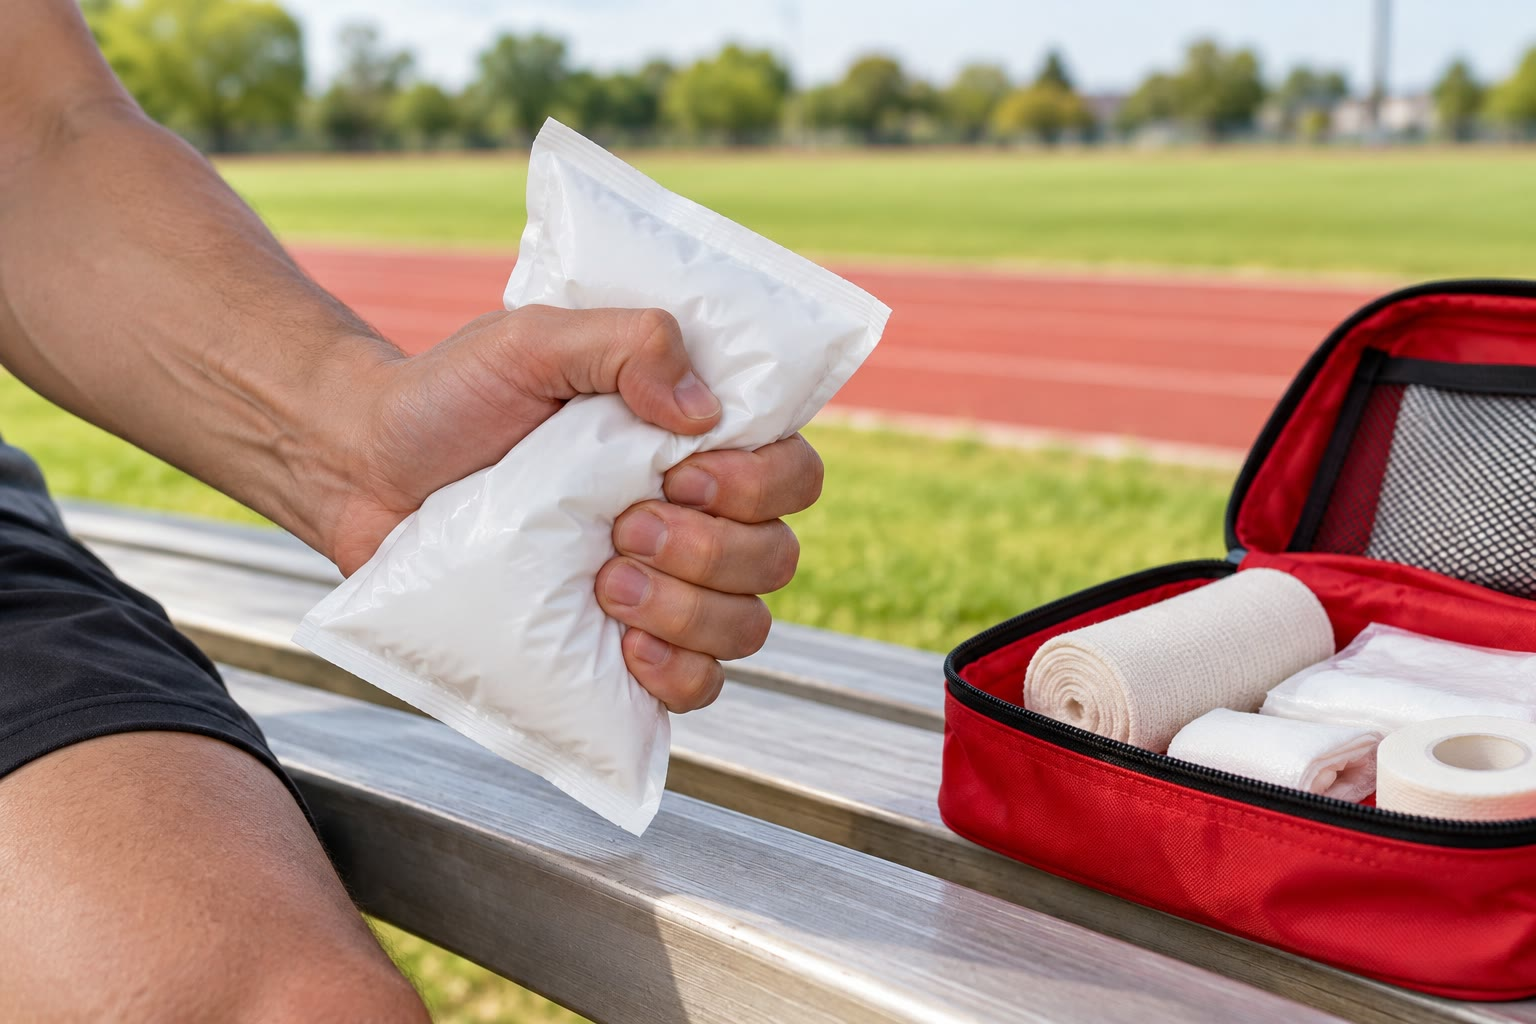
\includegraphics[width=0.55\linewidth]{images/book3/ai/b2-02-cold-pack.jpg}

{\small كمادة تبريد: حين يُكسر كيسها الداخلي تذوب نترات الأمونيوم في الماء
وتبرد الكمادة. الذوبان \omterm{def:b2:reaction-enthalpy:exothermic}{ماص للحرارة} وتلقائي معًا؛ وإنتروبياه تفسر السبب
(\cref{ex:b2:reaction-free-energy:cold-pack}).}
\end{omfigure}

\section{الإنتروبيات القياسية والمبدأ الثالث}

خلافًا للأنتالبي، للإنتروبيا صفر طبيعي.

\begin{theorem}[المبدأ الثالث في الترموديناميك]\label{thm:b2:reaction-free-energy:third-law}
تؤول إنتروبيا بلورة نقية تامة الانتظام إلى الصفر حين تؤول درجة حرارتها إلى
\qty{0}{K}.
\end{theorem}
\admitted

\begin{remark}[من أين يأتي الصفر]\label{rem:b2:reaction-free-energy:third-law}
نص فالتر نرنست سنة 1906 على أن إنتروبيات التفاعل بين أطوار مكثفة تنعدم
حين $T \to 0$؛ ثم صاغه ماكس بلانك بدقة أكبر في النص أعلاه. وأصله
إحصائي: فالإنتروبيا تعدّ الترتيبات المجهرية المتوافقة مع حالة النظام،
وللبلورة التامة عند \qty{0}{K} ترتيب واحد. ويجري هذا العدّ في مجلد السنة
الثالثة، بدوال التجزئة.
\end{remark}

\begin{definition}[الإنتروبيا المولية القياسية]\label{def:b2:reaction-free-energy:standard-entropy}
\emph{الإنتروبيا المولية القياسية}\index{إنتروبيا مولية قياسية}
$S^\circ_m(T)$ لمادة هي إنتروبيا مول واحد منها في حالتها القياسية عند درجة
الحرارة $T$، والصفر هو صفر المبدأ الثالث. وهي، خلافًا للمقدار
$\Delta_f H^\circ$، مقدار مطلق، موجب لكل مادة، والعناصر منها.
\end{definition}

\begin{proposition}[الإنتروبيا المطلقة من السعات الحرارية]\label{prop:b2:reaction-free-energy:absolute-entropy}
بتسخين مادة عند ضغط ثابت $p^\circ$ من \qty{0}{K} إلى $T$،
\[
  S^\circ_m(T) = \int_0^T\frac{C^\circ_{p,m}(T')}{T'}\,\dd T' +
  \sum_{\text{التحولات}}\frac{\Delta_{\text{تحول}}H^\circ}{T_{\text{تحول}}} ,
\]
حيث يؤخذ التكامل في كل طور على مجال درجات حرارته.
\end{proposition}

\begin{proof}
لنسخّن المادة تسخينًا عكوسًا عند ضغط ثابت: $\delta S_{\text{c}} =
0$ و$\delta Q = \dd H = C_p\,\dd T$، ومنه $\dd S = C_p\,\dd T/T$. وعند
تحوّل (انصهار، غليان) تبقى درجة الحرارة عند $T_{\text{تحول}}$
بينما تُستقبل الحرارة $\Delta_{\text{تحول}}H$ بطريقة عكوسة: فتقفز الإنتروبيا
بمقدار $\Delta_{\text{تحول}}H/T_{\text{تحول}}$. ثم تُجمع القطع انطلاقًا من
صفر المبدأ الثالث.
\end{proof}

\begin{omfigure}
\begin{tikzpicture}
\begin{axis}[
  width=0.8\linewidth, height=6.2cm, xmin=0, xmax=1500, ymin=0, ymax=210,
  axis x line=bottom, axis y line=left, xlabel={\babelsublr{$T$ (K)}},
  ylabel={\foreignlanguage{arabic}{$S^\circ_m$ للزنك \babelsublr{(\unit{J/(K.mol)})}}},
  xtick={0,250,500,750,1000,1250,1500},
  tick label style={font=\small}, label style={font=\small}, clip=false]
\addplot[omDef, very thick, smooth] table[x=T, y=S] {figdata/out/bachelor-2-standard-entropy-solid.dat};
\addplot[omProp, very thick] table[x=T, y=S] {figdata/out/bachelor-2-standard-entropy-liquid.dat};
\addplot[omThm, very thick] table[x=T, y=S] {figdata/out/bachelor-2-standard-entropy-gas.dat};
\draw[densely dashed, gray] (axis cs:692.73,64.6) -- (axis cs:692.73,75.2);
\draw[densely dashed, gray] (axis cs:1180.2,91.9) -- (axis cs:1180.2,189.6);
\node[omDef, font=\small, anchor=south east] at (axis cs:600,60) {صلب};
\node[omProp, font=\small, anchor=north west] at (axis cs:850,78) {سائل};
\node[omThm, font=\small, anchor=south] at (axis cs:1350,192) {غاز};
\node[font=\scriptsize, anchor=west, align=left] at (axis cs:700,110) {\foreignlanguage{arabic}{انصهار، $+10.6$}\\ \foreignlanguage{arabic}{عند \qty{692.7}{K}}};
\node[font=\scriptsize, anchor=east, align=right] at (axis cs:1170,150) {\foreignlanguage{arabic}{غليان،}\\ \foreignlanguage{arabic}{$+97.7$ عند}\\ \qty{1180.2}{K}};
\end{axis}
\end{tikzpicture}

{\small \omterm{def:b2:reaction-free-energy:standard-entropy}{الإنتروبيا المولية القياسية} للزنك انطلاقًا من صفر المبدأ الثالث. تزداد
مع درجة الحرارة إذ يختزن الفلز الحرارة، ثم تقفز عند نقطة الانصهار بمقدار
$\Delta_{\text{انصهار}}H/T_{\text{انصهار}}$، وبمقدار أكبر بكثير عند نقطة
الغليان، $\Delta_{\text{تبخر}}H/T_b$: فالغاز أشد فوضى بكثير من
السائل.}
% ledger: s0T:Zn_crl.0, s0T:Zn_crl.298.15, s0T:Zn_cr.692, s0T:Zn_l.692, s0T:Zn_l.1180, s0T:Zn_g.1180, hT:Zn_cr.692, hT:Zn_l.692, hT:Zn_l.1180, hT:Zn_g.1180, dfh:Zn_g (curve in figdata/bachelor-2/standard-entropy.py)
\end{omfigure}

يعطي الشكل رتب قدر جديرة بالحفظ. ففي درجة حرارة الغرفة يحمل الفلز أو
البلورة الصلبة بضع عشرات من \unit{J/(K.mol)}، والسائل نحو مئة، والغاز من
مئة إلى ثلاثمئة؛ والانصهار يضيف قليلًا، والغليان يضيف كثيرًا. والإنتروبيات
المولية القياسية المستعملة في هذا المجلد مجدولة مع أنتالبيات التكوين.

\section{إنتروبيا التفاعل}

\begin{definition}[إنتروبيا التفاعل]\label{def:b2:reaction-free-energy:reaction-entropy}
\emph{إنتروبيا التفاعل}\index{إنتروبيا التفاعل} هي $\Delta_r S =
(\partial S/\partial\xi)_{T,p}$، و\emph{إنتروبيا التفاعل
القياسية}\index{إنتروبيا التفاعل القياسية} هي $\Delta_r S^\circ(T) =
\sum_i\nu_iS^\circ_{m,i}(T)$، بوحدة \unit{J/(K.mol)}.
\end{definition}

لأن الإنتروبيات القياسية مطلقة، لا حاجة إلى أي تفاعل تكوين: فالعناصر تُحسب
بإنتروبياتها الخاصة.

\begin{example}[ثلاث إنتروبيات تفاعل]\label{ex:b2:reaction-free-energy:entropies}
عند \qty{298.15}{K}:
\begin{itemize}
  \item \ce{CaCO3(s) -> CaO(s) + CO2(g)}: $\Delta_r S^\circ = 39.75 + 213.79 -
        92.9 = \qty{+160.6}{J/(K.mol)}$، غاز يتكوّن من جسم صلب؛
  \item \ce{N2(g) + 3H2(g) -> 2NH3(g)}: $\Delta_r S^\circ = 2(192.77) -
        191.61 - 3(130.68) = \qty{-198.1}{J/(K.mol)}$، أربعة جزيئات غازية
        تصير جزيئين؛
  \item \ce{N2O4(g) -> 2NO2(g)}: $\Delta_r S^\circ = 2(240.03) - 304.38 =
        \qty{+175.7}{J/(K.mol)}$.
\end{itemize}
% ledger: s0:CaCO3_cr, s0:CaO_cr, s0:CO2_g, s0:N2_g, s0:H2_g, s0:NH3_g, s0:N2O4_g, s0:NO2_g (computed in figdata/bachelor-2/thermo-data.py)
\end{example}

\begin{proposition}[إشارة إنتروبيا التفاعل]\label{prop:b2:reaction-free-energy:sign-rule}
حين تشارك غازات في التفاعل، تكون إشارة $\Delta_r S^\circ$ عمومًا إشارة
$\Delta\nu_{\text{غاز}} = \sum_{\text{غازات}}\nu_i$، ويكون مقدارها نحو
\qty{100}{} إلى \qty{200}{J/(K.mol)} لكل مول من الغاز المتكوّن أو المستهلَك. وحين
يكون $\Delta\nu_{\text{غاز}} = 0$، أو لا يشارك أي غاز، يكون $\Delta_r S^\circ$
صغيرًا ويجب حساب إشارته.
\end{proposition}

\begin{proof}[تعليل]
الإنتروبيا المولية لغاز عند \qty{298}{K} بين 130 
و\qty{300}{J/(K.mol)}، وإنتروبيا الجسم الصلب أو السائل بضع عشرات: فتكوين مول
من الغاز أو استهلاكه يطغى على كل مساهمة أخرى. إنها قاعدة تجريبية، لا
مبرهنة: فذوبان ملح، دون أي غاز، قد يغيّر الإنتروبيا مع ذلك بنحو مئة
\unit{J/(K.mol)}.
\end{proof}

\begin{method}[التنبؤ بإشارة $\Delta_r S^\circ$]\label{met:b2:reaction-free-energy:entropy-sign}
\begin{enumerate}
  \item احسب $\Delta\nu_{\text{غاز}}$: إن لم يكن معدومًا فهو يعطي
        الإشارة.
  \item وإلا فقارن انتظام الحالات: إذابة بلورة، والانصهار، وكسر جزيء إلى
        قطعتين، كلها ترفع الإنتروبيا؛ والترسيب، والتجمد، وضم جزيئين في
        جزيء واحد، كلها تخفضها.
  \item حين يكون القرار مهمًا، احسب $\sum_i\nu_iS^\circ_{m,i}$.
\end{enumerate}
\end{method}

لقي مجلد السنة الأولى نتيجة لذلك: فالحذف يصنع جزيئات أكثر مما يصنعه
استبدال بالكواشف نفسها (الألكين والمجموعة المغادرة والقاعدة المبرتنة،
مقابل ناتج الاستبدال والمجموعة المغادرة). فإنتروبيا تفاعله أكبر، وحد
الإنتروبيا، الذي يكبر مع درجة الحرارة كما يبيّن القسم التالي، هو سبب
تفضيل الحرارة للحذف على الاستبدال.

\section{طاقة جيبس}

\begin{definition}[طاقة جيبس]\label{def:b2:reaction-free-energy:gibbs-energy}
\emph{طاقة جيبس}\index{طاقة جيبس} لنظام (أو أنتالبيه الحر) هي دالة الحالة
$G = H - TS$، وهي ممتدة، وتقاس بالجول.
\end{definition}

\begin{definition}[طاقة جيبس للتفاعل]\label{def:b2:reaction-free-energy:reaction-gibbs}
\emph{طاقة جيبس للتفاعل}\index{طاقة جيبس للتفاعل} هي $\Delta_r G
= (\partial G/\partial\xi)_{T,p}$، و\emph{طاقة جيبس القياسية
للتفاعل}\index{طاقة جيبس القياسية للتفاعل} هي $\Delta_r G^\circ(T) =
\sum_i\nu_iG^\circ_{m,i}(T)$، وكلتاهما بوحدة \unit{kJ/mol}.
\end{definition}

\begin{proposition}[حدّ الأنتالبي وحدّ الإنتروبيا]\label{prop:b2:reaction-free-energy:g-h-s}
$\Delta_r G = \Delta_r H - T\Delta_r S$، و$\Delta_r G^\circ = \Delta_r
H^\circ - T\Delta_r S^\circ$.
\end{proposition}

\begin{proof}
نشتق $G = H - TS$ بالنسبة إلى $\xi$ عند $T$ و$p$ ثابتين: فالمقدار $T$
ثابت في هذا الاشتقاق.
\end{proof}

\begin{proposition}[تفاضل $G$ لنظام متفاعل]\label{prop:b2:reaction-free-energy:dG}
من أجل نظام مغلق يجري فيه تفاعل واحد، عند $T$ و$p$
منتظمين،
\[
  \dd G = V\,\dd p - S\,\dd T + \Delta_r G\,\dd\xi .
\]
\end{proposition}

\begin{proof}
للدالة $G(T, p, \xi)$ التفاضل التام $\dd G = (\partial G/\partial
T)_{p,\xi}\dd T + (\partial G/\partial p)_{T,\xi}\dd p + \Delta_r G\,\dd\xi$.
والمشتقتان الجزئيتان الأوليان مأخوذتان عند تركيب ثابت: فهما مشتقتا نظام
مغلق ثابت التركيب، تعطي له الفيزياء
$\dd U = T\dd S - p\dd V$، بحيث $\dd G = \dd U + p\dd V + V\dd p - T\dd S
- S\dd T = V\dd p - S\dd T$. ومنه $(\partial G/\partial T)_{p,\xi} = -S$
و$(\partial G/\partial p)_{T,\xi} = V$.
\end{proof}

\section{محك التطور}

\begin{theorem}[محك التطور]\label{thm:b2:reaction-free-energy:evolution}
في نظام مغلق محفوظ عند درجة حرارة وضغط ثابتين، لا يتبادل شغلًا غير شغل
قوى الضغط، لا يمكن لتفاعل أن يتقدم إلا في الاتجاه الذي يجعل
\[
  \Delta_r G\,\dd\xi \leq 0 ,
\]
مع المساواة عند التوازن. فإذا كان $\Delta_r G < 0$ جرى التفاعل في
الاتجاه المباشر، وإذا كان $\Delta_r G > 0$ جرى في الاتجاه المعاكس، ويكون
النظام في توازن حين يكون $\Delta_r G = 0$.
\end{theorem}

\begin{proof}
لنأخذ تحوّلًا متناهي الصغر عند $T$ و$p$ منتظمين، مساويين لقيمتيهما في
الوسط المحيط. يعطي المبدأ الأول مع شغل الضغط وحده $\dd U = \delta Q
- p\dd V$؛ ويعطي الثاني $\delta Q = T\dd S - T\delta S_{\text{c}}$. ومنه
\[
  \dd G = \dd U + p\dd V + V\dd p - T\dd S - S\dd T = -T\,\delta
  S_{\text{c}} + V\dd p - S\dd T .
\]
وبالمقارنة مع \cref{prop:b2:reaction-free-energy:dG}، عند $T$ و$p$ ثابتين:
$\Delta_r G\,\dd\xi = -T\,\delta S_{\text{c}}$. ولأن $\delta S_{\text{c}}
\geq 0$، فإن $\Delta_r G\,\dd\xi \leq 0$، ويتطلب $\delta S_{\text{c}} = 0$
(تحوّل عكوس، تحوّل توازن) أن يكون $\Delta_r G = 0$.
\end{proof}

\begin{remark}[ما يقوله المحك وما لا يقوله]\label{rem:b2:reaction-free-energy:criterion}
الإنتروبيا التي يولّدها تفاعل عند $T$ و$p$ ثابتين هي $-\Delta_r G\,
\dd\xi/T$: \omterm{def:b2:reaction-free-energy:gibbs-energy}{فطاقة جيبس} هي المبدأ الثاني مقصورًا على ظروف المختبر ومكتوبًا
بمقادير النظام وحده. وهي تقول في أي اتجاه يمكن أن يسير التفاعل، ولا تقول
أبدًا بأي سرعة: فالألماس، الذي يكون لتحوّله إلى غرافيت $\Delta_r G^\circ < 0$،
يدوم إلى الأبد على خاتم. وهي تفترض غياب أي شغل آخر: فالخلية التي تعطي
شغلًا كهربائيًا، أو جهاز التحليل الكهربائي الذي يستقبله، يخضعان لمحك معدَّل
(\cref{ch:b2:cell-thermodynamics}).
\end{remark}

\begin{definition}[طارد للطاقة، ماص للطاقة]\label{def:b2:reaction-free-energy:exergonic}
يكون التفاعل \emph{طاردًا للطاقة}\index{طارد للطاقة} في حالة معيّنة حين يكون
$\Delta_r G < 0$، و\emph{ماصًا للطاقة}\index{ماص للطاقة} حين يكون $\Delta_r G >
0$. وحين يكون كل نوع كيميائي في حالته القياسية، تنطبق هاتان الكلمتان على
إشارة $\Delta_r G^\circ$.
\end{definition}

يستعمل المحك $\Delta_r G$، أي القيمة في الحالة الفعلية للنظام؛ أما
$\Delta_r G^\circ$ فيخص كل نوع كيميائي في حالته القياسية، وهي نادرًا ما تكون
حالة خليط حقيقي. والصلة بينهما، عبر التركيب، هي موضوع
\cref{ch:b2:chemical-potential}، وتعطي قانون السنة الأولى $Q = K^\circ$ في
\cref{ch:b2:equilibrium-shifts}. ومن أجل التفاعلات بين أجسام صلبة وسوائل
نقية، وغازات عند \qty{1}{bar}، تتطابق القيمتان.

\begin{example}[كمادة التبريد]\label{ex:b2:reaction-free-energy:cold-pack}
من أجل \ce{NH4NO3(s) -> NH4+(aq) + NO3-(aq)} عند \qty{298.15}{K}، في الحالات
القياسية: $\Delta_r H^\circ = -339.87 + 365.56 = \qty{+25.69}{kJ/mol}$
و$\Delta_r S^\circ = 259.8 - 151.08 = \qty{+108.7}{J/(K.mol)}$، ومنه
$\Delta_r G^\circ = 25.69 - 298.15 \times 0.1087 = \qty{-6.7}{kJ/mol}$: فالذوبان
\omterm{def:b2:reaction-enthalpy:exothermic}{ماص للحرارة} \omterm{def:b2:reaction-free-energy:exergonic}{وطارد للطاقة}. والأيونات، الحرة في الماء، أشد فوضى منها في
البلورة، وحد الإنتروبيا $T\Delta_r
S^\circ = \qty{32.4}{kJ/mol}$ يرجح على كلفة الأنتالبي.
% ledger: dfh:NH4NO3_cr, s0:NH4NO3_cr, dfh:NH4NO3_ai, s0:NH4NO3_ai (computed in figdata/bachelor-2/thermo-data.py)
\end{example}

\begin{history}[جوزايا ويلارد جيبس]
\begin{minipage}[t]{0.2\linewidth}\vspace{0pt}
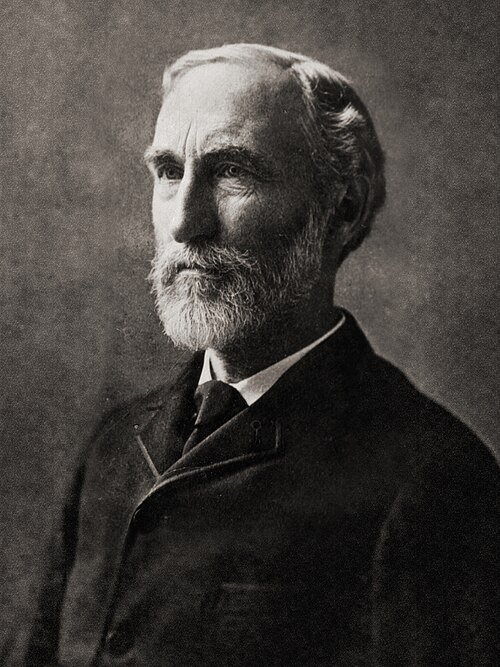
\includegraphics[width=\linewidth]{images/book3/gibbs.jpg}
\end{minipage}\hfill
\begin{minipage}[t]{0.76\linewidth}\vspace{0pt}
جوزايا ويلارد جيبس (1839--1903)، أستاذ الفيزياء الرياضية في جامعة ييل،
نشر بين 1876 و1878 بحثه \emph{في توازن المواد غير المتجانسة}، نحو
ثلاثمئة صفحة في محاضر أكاديمية صغيرة، تظهر فيها الطاقة الحرة والجهد
الكيميائي وقاعدة الأطوار التي تأتي في الفصول التالية. ولم يقرأه إلا قليل
من الكيميائيين إلى أن تُرجم في تسعينيات القرن التاسع عشر. (صورة: ملكية
عامة، ويكيميديا كومنز.)
\end{minipage}
\end{history}

\section{طاقات جيبس القياسية للتفاعل ودرجة الحرارة}

\begin{definition}[تقريب إلينغهام]\label{def:b2:reaction-free-energy:ellingham-approximation}
يعدّ \emph{تقريب إلينغهام}\index{تقريب إلينغهام} المقدارين
$\Delta_r H^\circ$ و$\Delta_r S^\circ$ مستقلين عن درجة الحرارة
على فترة لا تحوي أي تغيّر للحالة الفيزيائية. فتكون $\Delta_r G^\circ(T)
= \Delta_r H^\circ - T\Delta_r S^\circ$ مستقيمًا بدلالة $T$، ميله
$-\Delta_r S^\circ$.
\end{definition}

\begin{proposition}[المشتقات بالنسبة إلى درجة الحرارة]\label{prop:b2:reaction-free-energy:gibbs-helmholtz}
لدينا
\[
  \frac{\dd\Delta_r G^\circ}{\dd T} = -\Delta_r S^\circ, \qquad
  \frac{\dd}{\dd T}\!\left(\frac{\Delta_r G^\circ}{T}\right) =
  -\frac{\Delta_r H^\circ}{T^2}\ \ \text{(جيبس--هلمهولتز)}, \qquad
  \frac{\dd\Delta_r S^\circ}{\dd T} = \frac{\Delta_r C^\circ_p}{T}.
\]
وبخاصة يصح \omterm{def:b2:reaction-free-energy:ellingham-approximation}{تقريب إلينغهام} حين يكون $\Delta_r C^\circ_p$
صغيرًا.
\end{proposition}

\begin{proof}
وكل نوع كيميائي في حالته القياسية، يكون للدالة $G^\circ(T, \xi)$ أن $(\partial
G^\circ/\partial T)_\xi = -S^\circ$ (\cref{prop:b2:reaction-free-energy:dG}).
وحسب مبرهنة شفارتز،
\[
  \frac{\dd\Delta_r G^\circ}{\dd T} = \partial_\xi\partial_T G^\circ =
  -\partial_\xi S^\circ = -\Delta_r S^\circ .
\] ثم $\frac{\dd}{\dd
T}(\Delta_r G^\circ/T) = \frac{-T\Delta_r S^\circ - \Delta_r G^\circ}{T^2} =
-\frac{\Delta_r H^\circ}{T^2}$. وأخيرًا، $\dd S^\circ_m = C^\circ_{p,m}\,\dd
T/T$ لكل نوع كيميائي (\cref{prop:b2:reaction-free-energy:absolute-entropy})،
والتركيب نفسه يعطي العلاقة الأخيرة. وإذا كان $\Delta_r C^\circ_p$
صغيرًا، فإن $\Delta_r H^\circ$ (كيرشوف) و$\Delta_r S^\circ$ لا يكادان يتغيران.
\end{proof}

\begin{definition}[درجة حرارة الانقلاب]\label{def:b2:reaction-free-energy:inversion-temperature}
حين تكون إشارتا $\Delta_r H^\circ$ و$\Delta_r S^\circ$ متماثلتين، تكون
\emph{درجة حرارة الانقلاب}\index{درجة حرارة الانقلاب} للتفاعل هي
درجة الحرارة التي تتغير عندها إشارة $\Delta_r G^\circ$؛ وفي \omterm{def:b2:reaction-free-energy:ellingham-approximation}{تقريب إلينغهام}،
$T_i = \Delta_r H^\circ/\Delta_r S^\circ$.
\end{definition}

\begin{omfigure}
\begin{tikzpicture}
\begin{axis}[
  width=0.72\linewidth, height=5.6cm, xmin=0, xmax=1600, ymin=0, ymax=260,
  axis x line=bottom, axis y line=left, xlabel={\babelsublr{$T$ (K)}}, ylabel={\babelsublr{\unit{kJ/mol}}},
  tick label style={font=\small}, label style={font=\small}, clip=false]
\addplot[omThm, very thick] table[x=T, y=DrH] {figdata/out/bachelor-2-thermo-data-calcite.dat};
\addplot[omDef, very thick] table[x=T, y=TDrS] {figdata/out/bachelor-2-thermo-data-calcite.dat};
\node[omThm, anchor=south west, font=\small] at (axis cs:60,180) {$\Delta_r H^\circ = 178.3$};
\node[omDef, anchor=west, font=\small] at (axis cs:1600,257) {$T\Delta_r S^\circ$};
\draw[dotted] (axis cs:1110,0) -- (axis cs:1110,178.3);
\node[anchor=south west, font=\small] at (axis cs:1120,8) {$T_i = \qty{1110}{K}$};
\node[font=\scriptsize, align=center] at (axis cs:600,140) {$\Delta_r G^\circ > 0$:\\ \foreignlanguage{arabic}{الكالسيت مستقر}};
\node[font=\scriptsize, align=center] at (axis cs:1470,206) {$\Delta_r G^\circ < 0$};
\end{axis}
\end{tikzpicture}

{\small حدّا الأنتالبي والإنتروبيا للتفاعل \ce{CaCO3(s) -> CaO(s) + CO2(g)}
في \omterm{def:b2:reaction-free-energy:ellingham-approximation}{تقريب إلينغهام}. تحت \omterm{def:b2:reaction-free-energy:inversion-temperature}{درجة حرارة الانقلاب} تغلب كلفة الأنتالبي ويكون
الحجر الجيري مستقرًا تحت \qty{1}{bar} من ثنائي أكسيد الكربون؛ وفوقها يغلب حد
الإنتروبيا فيتفكك الحجر الجيري.}
% ledger: dfh:CaCO3_cr, dfh:CaO_cr, dfh:CO2, s0:CaCO3_cr, s0:CaO_cr, s0:CO2_g (computed in figdata/bachelor-2/thermo-data.py)
\end{omfigure}

\begin{omfigure}
\begin{tikzpicture}[font=\small]
  \draw[thick] (0,0) rectangle (8,4);
  \draw[thick] (4,0) -- (4,4) (0,2) -- (8,2);
  \node[above] at (2,4) {$\Delta_r H^\circ < 0$};
  \node[above] at (6,4) {$\Delta_r H^\circ > 0$};
  \node[left] at (0,3) {$\Delta_r S^\circ > 0$};
  \node[left] at (0,1) {$\Delta_r S^\circ < 0$};
  \node[align=center, omDef] at (2,3) {\foreignlanguage{arabic}{طارد للطاقة}\\ \foreignlanguage{arabic}{عند كل $T$}};
  \node[align=center, omProp] at (6,3) {\foreignlanguage{arabic}{طارد للطاقة}\\ \foreignlanguage{arabic}{فوق $T_i$}};
  \node[align=center, omProp] at (2,1) {\foreignlanguage{arabic}{طارد للطاقة}\\ \foreignlanguage{arabic}{تحت $T_i$}};
  \node[align=center, omThm] at (6,1) {\foreignlanguage{arabic}{ماص للطاقة}\\ \foreignlanguage{arabic}{عند كل $T$}};
\end{tikzpicture}

{\small الحالات الأربع للعلاقة $\Delta_r G^\circ = \Delta_r H^\circ - T\Delta_r
S^\circ$ (\omterm{def:b2:reaction-free-energy:ellingham-approximation}{تقريب إلينغهام}). الاحتراقات في الخانة العليا اليسرى؛ وتفكك الحجر
الجيري وكمادة التبريد في العليا اليمنى؛ وتخليق الأمونيا في السفلى
اليسرى.}
\end{omfigure}

\begin{method}[طاقة جيبس القياسية لتفاعل عند درجة الحرارة $T$]\label{met:b2:reaction-free-energy:delta-g-standard}
\begin{enumerate}
  \item انطلاقًا من الجداول عند \qty{298.15}{K}، احسب $\Delta_r H^\circ$
        و$\Delta_r S^\circ$.
  \item تحقق من أن أي نوع كيميائي لا يغيّر حالته الفيزيائية بين \qty{298}{K}
        و$T$؛ وإلا فأضف التحوّل (أنتالبيه وإنتروبياه) أو انطلق من الحالة
        الجديدة.
  \item في \omterm{def:b2:reaction-free-energy:ellingham-approximation}{تقريب إلينغهام}، $\Delta_r G^\circ(T) = \Delta_r H^\circ
        - T\Delta_r S^\circ$.
  \item حين لا يكون $\Delta_r C^\circ_p$ صغيرًا أو تكون الفترة طويلة،
        استعمل مباشرة قيم $\Delta_f G^\circ(T)$ المجدولة.
\end{enumerate}
\end{method}

\begin{example}[اختباران للتقريب]\label{ex:b2:reaction-free-energy:tests}
للحجر الجيري، $\Delta_r C^\circ_p = 42.80 + 37.13 - 81.88 =
\qty{-2.0}{J/(K.mol)}$: فالتقريب ممتاز، و$\Delta_r
G^\circ = 178.3 - T \times 0.1606$ تعطي $T_i = \qty{1110}{K}$. وللأمونيا،
$\Delta_r G^\circ(700) \approx -91.9 + 700 \times 0.1981 =
\qty{+46.8}{kJ/mol}$، في حين تعطي الجداول $2\Delta_f G^\circ(\ce{NH3}, 700) =
\qty{+54.4}{kJ/mol}$: فهنا $\Delta_r C^\circ_p = \qty{-44}{J/(K.mol)}$ والخطأ
\qty{8}{kJ/mol}، أي عامل 4 على ثابت التوازن عند درجة الحرارة
تلك.
% ledger: cp:CaO_cr.298, cp:CO2_g.298, cp:CaCO3_cr.298, janafG:NH3.700 (computed in figdata/bachelor-2/thermo-data.py)
\end{example}

\section{تمارين}

\begin{exercise}[$\star$]\label{exo:b2:reaction-free-energy:1}
تنبأ بإشارة $\Delta_r S^\circ$ في: (أ) \ce{2H2(g) + O2(g) -> 2H2O(l)}؛
(ب) \ce{CaCO3(s) -> CaO(s) + CO2(g)}؛ (ج) \ce{N2O4(g) -> 2NO2(g)}؛
(د) \ce{Ag+(aq) + Cl-(aq) -> AgCl(s)}؛ (ه) \ce{H2O(s) -> H2O(l)}؛
(و) \ce{H2(g) + Cl2(g) -> 2HCl(g)}.
\end{exercise}

\begin{exercise}[$\star$]\label{exo:b2:reaction-free-energy:2}
احسب $\Delta_r S^\circ$ و$\Delta_r G^\circ$ عند \qty{298.15}{K} لتخليق
الأمونيا، \ce{N2(g) + 3H2(g) -> 2NH3(g)}، مع $\Delta_r
H^\circ = \qty{-91.9}{kJ/mol}$ وإنتروبيات الفصل. هل هو \omterm{def:b2:reaction-free-energy:exergonic}{طارد
للطاقة}؟
\end{exercise}

\begin{exercise}[$\star$]\label{exo:b2:reaction-free-energy:3}
احسب $\Delta_r G^\circ(\qty{298.15}{K})$ للتفاعل \ce{H2(g) + 1/2O2(g) ->
H2O(l)} انطلاقًا من $\Delta_f H^\circ(\ce{H2O}, \text{l}) = \qty{-285.83}{kJ/mol}$
والإنتروبيات القياسية \ce{H2(g)} 130.68، \ce{O2(g)} 205.15،
\ce{H2O(l)} \qty{69.95}{J/(K.mol)}. لماذا تكون هذه القيمة \omterm{def:b2:reaction-free-energy:reaction-gibbs}{طاقة جيبس القياسية}
لتكوين الماء السائل؟
% ledger: dfh:H2O-l, s0:H2_g, s0:O2_g, s0:H2O_l
\end{exercise}

\begin{exercise}[$\star$]\label{exo:b2:reaction-free-energy:4}
استعمل شكل إنتروبيا الزنك لقراءة إنتروبياه المولية القياسية عند
\qty{298}{K} وعند \qty{1000}{K}، وقفزتيها عند نقطتي الانصهار والغليان.
واستنتج أنتالبيي انصهاره وتبخره.
\end{exercise}

\begin{exercise}[$\star\star$]\label{exo:b2:reaction-free-energy:5}
من أجل \ce{H2O(l) -> H2O(g)} عند \qty{298.15}{K}، احسب $\Delta_r H^\circ$
و$\Delta_r S^\circ$ و$\Delta_r G^\circ$ من جداول الفصل.
فسّر لماذا $\Delta_r S^\circ \neq \Delta_r H^\circ/T$ عند \qty{298}{K}، وما
يعنيه كون $\Delta_r G^\circ$ موجبًا، وقدّر في \omterm{def:b2:reaction-free-energy:ellingham-approximation}{تقريب إلينغهام}
درجة الحرارة التي يكون عندها الماء السائل وبخاره عند
\qty{1}{bar} في توازن. وقارن بنقطة الغليان.
\end{exercise}

\begin{exercise}[$\star\star$]\label{exo:b2:reaction-free-energy:6}
من أجل \ce{N2O4(g) -> 2NO2(g)}، $\Delta_r H^\circ = \qty{57.1}{kJ/mol}$
و$\Delta_r S^\circ = \qty{175.7}{J/(K.mol)}$. احسب \omterm{def:b2:reaction-free-energy:inversion-temperature}{درجة حرارة الانقلاب}،
وفسّر لماذا يبهت لون أنبوب مختوم من الغاز البني \ce{NO2}
حين يُبرَّد في الجليد.
\end{exercise}

\begin{exercise}[$\star\star$]\label{exo:b2:reaction-free-energy:7}
لتفاعلٍ $\Delta_r G^\circ = \qty{-12.0}{kJ/mol}$ عند \qty{300}{K}
و$\qty{-4.0}{kJ/mol}$ عند \qty{400}{K}. أوجد في \omterm{def:b2:reaction-free-energy:ellingham-approximation}{تقريب إلينغهام}
$\Delta_r H^\circ$ و$\Delta_r S^\circ$، وتحقق من علاقة
جيبس--هلمهولتز.
\end{exercise}

\begin{exercise}[$\star\star$]\label{exo:b2:reaction-free-energy:8}
احسب $\Delta_r G^\circ$ لتكوين الميثان، \ce{C(s) + 2H2(g) ->
CH4(g)}، عند \qty{298.15}{K}، انطلاقًا من $\Delta_f H^\circ = \qty{-74.87}{kJ/mol}$
والإنتروبيات \ce{C} (غرافيت) 5.74، \ce{H2} 130.68، \ce{CH4}
\qty{186.25}{J/(K.mol)}. فوق أي درجة حرارة يصير الميثان غير مستقر بالنسبة
إلى عناصره تحت الضغط القياسي؟
% ledger: dfh:CH4_g, s0:C_gr, s0:H2_g, s0:CH4_g
\end{exercise}

\begin{exercise}[$\star\star$]\label{exo:b2:reaction-free-energy:9}
يتفاعل ألكان مهلجن مع قاعدة بالاستبدال أو بالحذف. اكتب التفاعلين كليهما
للمركب 2-برومو بروبان مع أيون الهيدروكسيد. ومع $\Delta_r
H^\circ(\text{حذف}) - \Delta_r H^\circ(\text{استبدال}) =
\qty{+40}{kJ/mol}$ و$\Delta_r S^\circ(\text{حذف}) - \Delta_r
S^\circ(\text{استبدال}) = \qty{+90}{J/(K.mol)}$ (رتب قدر)،
أوجد درجة الحرارة التي يصير فوقها الحذف الأكثر طردًا للطاقة بين
التفاعلين، وفسّر دور عدد الجزيئات.
\end{exercise}

\begin{exercise}[$\star\star\star$]\label{exo:b2:reaction-free-energy:10}
لا يبلغ أحادي أكسيد الكربون البلوري إنتروبيا معدومة عند \qty{0}{K}: فكل
جزيء يمكن أن يتموضع على هيئة CO أو OC بشكل شبه عشوائي، إذ للتوجهين طاقتان
متقاربتان جدًا. بقبول صيغة بولتزمان $S = k_B\ln W$، حيث
$W$ عدد الترتيبات (الذي يُعدّ في مجلد السنة الثالثة)، احسب
الإنتروبيا المولية المتبقية. لماذا لا ينطبق المبدأ الثالث على هذه
البلورة؟
\end{exercise}

\begin{exercise}[$\star\star\star$]\label{exo:b2:reaction-free-energy:11}
بيّن أنه إذا كان $\Delta_r C^\circ_p$ ثابتًا $c$، فإن
$\Delta_r S^\circ(T) = \Delta_r S^\circ(T_0) + c\ln(T/T_0)$ 
و$\Delta_r G^\circ(T) = \Delta_r H^\circ(T_0) - T\Delta_r S^\circ(T_0) +
c\,[T - T_0 - T\ln(T/T_0)]$. وطبّق ذلك على الحجر الجيري ($c =
\qty{-2.0}{J/(K.mol)}$) عند \qty{1100}{K}، وقِس خطأ
\omterm{def:b2:reaction-free-energy:ellingham-approximation}{تقريب إلينغهام}.
\end{exercise}

\begin{exercise}[$\star\star\star$]\label{exo:b2:reaction-free-energy:12}
يُصنع التيتانيوم من أكسيده، الروتيل، مرورًا بكلوريده. (أ) احسب
$\Delta_r H^\circ$ و$\Delta_r S^\circ$ عند \qty{298}{K} للتفاعل \ce{TiO2(s) +
2Cl2(g) -> TiCl4(g) + O2(g)}، مع \ce{TiO2} ($-944.0$ \unit{kJ/mol}،
\qty{50.62}{J/(K.mol)}) و\ce{TiCl4(g)} ($-763.2$، 353.2)، ثم
$\Delta_r G^\circ$ عند \qty{1000}{K} في \omterm{def:b2:reaction-free-energy:ellingham-approximation}{تقريب إلينغهام}.
(ب) يُضاف الكربون: \ce{C(s) + O2(g) -> CO2(g)}، $\Delta_r H^\circ =
\qty{-393.5}{kJ/mol}$، $\Delta_r S^\circ = \qty{+2.9}{J/(K.mol)}$. احسب
$\Delta_r G^\circ(\qty{1000}{K})$ لمجموع التفاعلين وفسّر كيف يدفع
التفاعلُ الثاني الأولَ.
% ledger: dfh:TiO2_cr, s0:TiO2_cr, dfh:TiCl4_g, s0:TiCl4_g, s0:Cl2_g, s0:O2_g, s0:C_gr, s0:CO2_g
\end{exercise}

\section{مسألة: فرن الجير}

\begin{problem}[{مسألة نهاية الأسبوع --- إنتروبيا تفكك وأنتالبيه، وطاقة
جيبس له بدلالة درجة الحرارة، ومحك التطور في فرن، والطاقة وثنائي أكسيد
الكربون لطن من الجير}]
\label{pb:b2:reaction-free-energy:1}
يُصنع الجير، \ce{CaO}، بتسخين الحجر الجيري، \ce{CaCO3}، في فرن. معطيات عند
\qty{298.15}{K}: $\Delta_f H^\circ$ (\unit{kJ/mol}) \ce{CaCO3(s)}
$-1206.92$، \ce{CaO(s)} $-635.09$، \ce{CO2(g)} $-393.51$؛ $S^\circ_m$
(\unit{J/(K.mol)}) 92.9، 39.75، 213.79؛ $C^\circ_{p,m}$ (\unit{J/(K.mol)})
81.88، 42.80، 37.13. الكتل المولية: \ce{CaO} \qty{56.08}{g/mol}، \ce{CO2}
\qty{44.01}{g/mol}، \ce{CH4} \qty{16.04}{g/mol}؛ احتراق الميثان، والماء
بخار، $\Delta_r H^\circ = \qty{-802.3}{kJ/mol}$.
% ledger: dfh:CaCO3_cr, dfh:CaO_cr, dfh:CO2, s0:CaCO3_cr, s0:CaO_cr, s0:CO2_g, cp:CaCO3_cr.298, cp:CaO_cr.298, cp:CO2_g.298

\medskip
\noindent\textbf{الجزء الأول --- في درجة حرارة الغرفة.}
\begin{enumerate}
  \item اكتب معادلة تفكك الحجر الجيري.
  \item احسب $\Delta_r H^\circ(\qty{298}{K})$. هل التفاعل \omterm{def:b2:reaction-enthalpy:exothermic}{ناشر للحرارة}؟
  \item احسب $\Delta_r S^\circ(\qty{298}{K})$ وفسّر إشارتها.
  \item احسب $\Delta_r G^\circ(\qty{298}{K})$.
  \item هل الحجر الجيري مستقر في درجة حرارة الغرفة تحت \qty{1}{bar} من
        ثنائي أكسيد الكربون؟ لماذا تدوم الجروف الكلسية؟
  \item احسب $\Delta_r C^\circ_p$، وبيّن ما يعنيه ذلك لتعلق
        $\Delta_r H^\circ$ و$\Delta_r S^\circ$ بدرجة الحرارة.
\end{enumerate}

\medskip
\noindent\textbf{الجزء الثاني --- التسخين.}
\begin{enumerate}[resume]
  \item اكتب $\Delta_r G^\circ(T)$ في \omterm{def:b2:reaction-free-energy:ellingham-approximation}{تقريب إلينغهام}.
  \item احسبها عند \qty{1000}{K} وعند \qty{1300}{K}.
  \item احسب \omterm{def:b2:reaction-free-energy:inversion-temperature}{درجة حرارة الانقلاب} $T_i$.
  \item تحقق من علاقة جيبس--هلمهولتز على هذه العبارة.
  \item قدّر، بصيغة \cref{exo:b2:reaction-free-energy:11}،
        تغيّر $\Delta_r G^\circ$ عند $T_i$ الناتج عن
        $\Delta_r C^\circ_p$، والانزياح الناتج في $T_i$.
\end{enumerate}

\medskip
\noindent\textbf{الجزء الثالث --- الفرن.}
في هذا الجزء يكون ثنائي أكسيد الكربون فوق الأجسام الصلبة عند \qty{1}{bar}،
بحيث $\Delta_r G = \Delta_r G^\circ$.
\begin{enumerate}[resume]
  \item ماذا يقول محك التطور عند \qty{1000}{K}؟ وعند
        \qty{1300}{K}؟
  \item ماذا يحدث لخليط من الجير وثنائي أكسيد الكربون عند
        \qty{1}{bar} يُبرَّد تحت $T_i$؟
  \item ما مقدار الإنتروبيا المتولدة لكل مول من الحجر الجيري يتفكك عند
        \qty{1300}{K}؟
  \item تكنس غازاتُ الاحتراق الأفرانَ، وهي أفقر في ثنائي أكسيد الكربون.
        خمّن، قبل الفصل التالي، هل يساعد ذلك على
        التفكك.
\end{enumerate}

\medskip
\noindent\textbf{الجزء الرابع --- طن من الجير.}
\begin{enumerate}[resume]
  \item احسب كمية مادة الجير في طن واحد.
  \item احسب الحرارة التي يمتصها التفاعل لكل طن من الجير
        (خذ $\Delta_r H^\circ$ ثابتًا).
  \item احسب كتلة ثنائي أكسيد الكربون التي يطلقها الحجر الجيري لكل
        طن من الجير.
  \item تأتي الحرارة من حرق الميثان بكفاءة نافعة قدرها
        50\,\%. احسب كتلة الميثان المحروق لكل طن من الجير.
  \item احسب ثنائي أكسيد الكربون الناتج عن هذا الميثان.
  \item احسب مجموع ثنائي أكسيد الكربون لكل طن من الجير، والحصة التي
        يعود سببها إلى الحجر الجيري نفسه.
  \item لماذا لا يمكن لوقود أنظف أن يخفض إلا جزءًا من هذه الانبعاثات؟
  \item اذكر درجة الحرارة التي يتفكك فوقها الحجر الجيري تحت
        \qty{1}{bar} من ثنائي أكسيد الكربون.
\end{enumerate}
\end{problem}
